\section{Image mask}
\label{sec:imask}

\subsection{The object {\tt Rox\_Imask}}
\label{sse:imask_object}

The image structures of {\bf \rox} can be coupled with an image mask structure \lstinline$Rox_Imask_Structure$ that contains a mask. % represented as a byte (unsigned char) tab. 

A mask can be declared using the pointer \lstinline$Rox_Imask$ to a \lstinline$Rox_Imask_Structure$:
 
\begin{lstlisting}
typedef struct Rox_Imask_Struct* Rox_Imask;
\end{lstlisting}

\subsection{Creating/Deleting a {\tt Rox\_Imask}}
\label{sse:creating_imask}
Functions are provided to allocate and deallocate a \lstinline$Rox_Imask$ object~:

\begin{lstlisting}
Rox_Error rox_imask_new(Rox_Imask * imask, Rox_Uint cols, Rox_Uint rows);
\end{lstlisting}
The \lstinline$rox_imask_new$ function allocates memory for a mask object. In this case, the size of allocated memory depends on parameters `cols' and `rows'.\\ 

The \lstinline$rox_imask_del$ function deallocates memory for a mask object. 
\begin{lstlisting}
Rox_Error rox_imask_del(Rox_Imask * M);
\end{lstlisting}
It is necessary to call this function when the structure is not used anymore.

\subsection{Main functions related to {\tt Rox\_Imask}}
\label{sse:imask_methods}

To each pixel of an image corresponds a mask information. If a mask byte is set to 0 (zero), then the corresponding pixel shall be ignored. If a mask byte is set to $\sim$0 (bitwise complement to zero), then the corresponding pixel shall be considered.  By default, an image mask is fully set to  $\sim$0 (bitwise complement to zero). \\

The user can easily define his own mask for a given image. The main
application in the tracking algorithm is to define a non-rectangular
reference region. For example, it is possible to define a circle where
all mask bytes inside this circle are set to  $\sim$0 (bitwise complement to zero) and all
others to 0 (zero). Thus the region to track is not a rectangle but a
circle, even if the image structure represents a rectangular region of
interest.\\

The user can create his own functions to set the image mask as he
wants. The only thing to do is to set to 0 the mask bytes
corresponding to ignored pixels and to  $\sim$0 (bitwise complement to zero) all the others.\\

A function is available to fill a mask object with user defined data~:

\begin{lstlisting}
void rox_imask_set_user(Rox_Imask imask, const Rox_Uchar* data);
\end{lstlisting}

\noindent The `imask' parameter is a \lstinline$Rox_Imask$ structure already allocated with \lstinline$rox_imask_new$. 
The second parameter contains the mask values defined by the user. \\

\noindent The following functions are provided to create basic masks:
\begin{description}
  \item[rox\_imask\_set\_zero]~: Sets the mask values to zero.
  \item[rox\_imask\_set\_one]~: Sets the mask values to one.
  \item[rox\_imask\_set\_ellipse]~: Sets a mask with elliptic shape.
%  \item[rox\_imask\_set\_polygon]~: Sets the image mask inside a polygon .
\end{description}

\noindent Example of mask objects settings~:
\begin{lstlisting}
{
  // Create and allocate Rox_Imask structures
  Rox_Uint size = 64; // The mask will be square
  Rox_Imask Ellipse = rox_imask_new(size, size);
  Rox_Imask User_defined = rox_imask_new(size, size);
  Rox_Imask Polygon = rox_imask_new(size, size);
  Rox_Imask Combination = rox_imask_new(size, size);
 
  // Data for the mask defined by the user
  Rox_Uchar Data[size * size];

  // Initialize Data
  for(int i = 0; i<size; i++)
  {
    for(int j = 0; j<size; j++)
	Data[i+j*size] = ~0;
  }

  for(int i = size/2; i<size; i++)
  {
    for(int j = 0; j<size/2; j++)
	Data[i+j*size] = 0;
  }

  for(int i = 0; i<size/2; i++)
  {
    for(j = size/2; j<size; j++)
	Data[i+j*size] = 0;
  }
   
  //Initialize points for polygon data (In this example, it is a triangle)
  const Rox_Uint points [6] = { 4, 3, 50, 32, 14, 57}; 

  // Set Masks
  rox_imask_set_ellipse(Ellipse);
  rox_imask_set_user(User_defined, Data);
  rox_imask_set_polygon(Polygon, points, 3);
  rox_imask_set_and(Combination, Polygon, User_defined);

  // Save masks
  rox_imask_savepgm("Ellipse.pgm", Ellipse);
  rox_imask_savepgm("User.pgm", User_defined);  
  rox_imask_savepgm("Combination.pgm", Combination);
  rox_imask_savepgm("Polygon.pgm", Polygon);

  // Free Memory
  rox_imask_del(User_defined);
  rox_imask_del(Ellipse);
  rox_imask_del(Polygon);
  rox_imask_del(Combination);
}
\end{lstlisting}

In the figure \ref{fig:mask}, you can see the example results.
In order of appearance, the masks are: Ellipse, User, User-Ellipse combination and Polygon. 
\begin{figure}[htbp] 
\begin{center}
 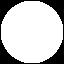
\includegraphics[width=0.24\textwidth]{vision/figures/Ellipse}  
 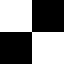
\includegraphics[width=0.24\textwidth]{vision/figures/User}  
 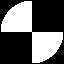
\includegraphics[width=0.24\textwidth]{vision/figures/And}
 
\includegraphics[width=0.24\textwidth]{vision/figures/Polygon}  \\ 
 \caption{Examples of setting masks.}
\label{fig:mask}
\end{center}
\end{figure} 
